% Generated by Sphinx.
\def\sphinxdocclass{report}
\documentclass[letterpaper,10pt,english]{sphinxmanual}
\usepackage[utf8]{inputenc}
\DeclareUnicodeCharacter{00A0}{\nobreakspace}
\usepackage{cmap}
\usepackage[T1]{fontenc}
\usepackage{babel}
\usepackage{times}
\usepackage[Bjarne]{fncychap}
\usepackage{longtable}
\usepackage{sphinx}
\usepackage{multirow}


\title{Stitch-seq-tools Documentation}
\date{September 27, 2013}
\release{1.0.1}
\author{Pengfei Yu}
\newcommand{\sphinxlogo}{}
\renewcommand{\releasename}{Release}
\makeindex

\makeatletter
\def\PYG@reset{\let\PYG@it=\relax \let\PYG@bf=\relax%
    \let\PYG@ul=\relax \let\PYG@tc=\relax%
    \let\PYG@bc=\relax \let\PYG@ff=\relax}
\def\PYG@tok#1{\csname PYG@tok@#1\endcsname}
\def\PYG@toks#1+{\ifx\relax#1\empty\else%
    \PYG@tok{#1}\expandafter\PYG@toks\fi}
\def\PYG@do#1{\PYG@bc{\PYG@tc{\PYG@ul{%
    \PYG@it{\PYG@bf{\PYG@ff{#1}}}}}}}
\def\PYG#1#2{\PYG@reset\PYG@toks#1+\relax+\PYG@do{#2}}

\expandafter\def\csname PYG@tok@gd\endcsname{\def\PYG@tc##1{\textcolor[rgb]{0.63,0.00,0.00}{##1}}}
\expandafter\def\csname PYG@tok@gu\endcsname{\let\PYG@bf=\textbf\def\PYG@tc##1{\textcolor[rgb]{0.50,0.00,0.50}{##1}}}
\expandafter\def\csname PYG@tok@gt\endcsname{\def\PYG@tc##1{\textcolor[rgb]{0.00,0.27,0.87}{##1}}}
\expandafter\def\csname PYG@tok@gs\endcsname{\let\PYG@bf=\textbf}
\expandafter\def\csname PYG@tok@gr\endcsname{\def\PYG@tc##1{\textcolor[rgb]{1.00,0.00,0.00}{##1}}}
\expandafter\def\csname PYG@tok@cm\endcsname{\let\PYG@it=\textit\def\PYG@tc##1{\textcolor[rgb]{0.25,0.50,0.56}{##1}}}
\expandafter\def\csname PYG@tok@vg\endcsname{\def\PYG@tc##1{\textcolor[rgb]{0.73,0.38,0.84}{##1}}}
\expandafter\def\csname PYG@tok@m\endcsname{\def\PYG@tc##1{\textcolor[rgb]{0.13,0.50,0.31}{##1}}}
\expandafter\def\csname PYG@tok@mh\endcsname{\def\PYG@tc##1{\textcolor[rgb]{0.13,0.50,0.31}{##1}}}
\expandafter\def\csname PYG@tok@cs\endcsname{\def\PYG@tc##1{\textcolor[rgb]{0.25,0.50,0.56}{##1}}\def\PYG@bc##1{\setlength{\fboxsep}{0pt}\colorbox[rgb]{1.00,0.94,0.94}{\strut ##1}}}
\expandafter\def\csname PYG@tok@ge\endcsname{\let\PYG@it=\textit}
\expandafter\def\csname PYG@tok@vc\endcsname{\def\PYG@tc##1{\textcolor[rgb]{0.73,0.38,0.84}{##1}}}
\expandafter\def\csname PYG@tok@il\endcsname{\def\PYG@tc##1{\textcolor[rgb]{0.13,0.50,0.31}{##1}}}
\expandafter\def\csname PYG@tok@go\endcsname{\def\PYG@tc##1{\textcolor[rgb]{0.20,0.20,0.20}{##1}}}
\expandafter\def\csname PYG@tok@cp\endcsname{\def\PYG@tc##1{\textcolor[rgb]{0.00,0.44,0.13}{##1}}}
\expandafter\def\csname PYG@tok@gi\endcsname{\def\PYG@tc##1{\textcolor[rgb]{0.00,0.63,0.00}{##1}}}
\expandafter\def\csname PYG@tok@gh\endcsname{\let\PYG@bf=\textbf\def\PYG@tc##1{\textcolor[rgb]{0.00,0.00,0.50}{##1}}}
\expandafter\def\csname PYG@tok@ni\endcsname{\let\PYG@bf=\textbf\def\PYG@tc##1{\textcolor[rgb]{0.84,0.33,0.22}{##1}}}
\expandafter\def\csname PYG@tok@nl\endcsname{\let\PYG@bf=\textbf\def\PYG@tc##1{\textcolor[rgb]{0.00,0.13,0.44}{##1}}}
\expandafter\def\csname PYG@tok@nn\endcsname{\let\PYG@bf=\textbf\def\PYG@tc##1{\textcolor[rgb]{0.05,0.52,0.71}{##1}}}
\expandafter\def\csname PYG@tok@no\endcsname{\def\PYG@tc##1{\textcolor[rgb]{0.38,0.68,0.84}{##1}}}
\expandafter\def\csname PYG@tok@na\endcsname{\def\PYG@tc##1{\textcolor[rgb]{0.25,0.44,0.63}{##1}}}
\expandafter\def\csname PYG@tok@nb\endcsname{\def\PYG@tc##1{\textcolor[rgb]{0.00,0.44,0.13}{##1}}}
\expandafter\def\csname PYG@tok@nc\endcsname{\let\PYG@bf=\textbf\def\PYG@tc##1{\textcolor[rgb]{0.05,0.52,0.71}{##1}}}
\expandafter\def\csname PYG@tok@nd\endcsname{\let\PYG@bf=\textbf\def\PYG@tc##1{\textcolor[rgb]{0.33,0.33,0.33}{##1}}}
\expandafter\def\csname PYG@tok@ne\endcsname{\def\PYG@tc##1{\textcolor[rgb]{0.00,0.44,0.13}{##1}}}
\expandafter\def\csname PYG@tok@nf\endcsname{\def\PYG@tc##1{\textcolor[rgb]{0.02,0.16,0.49}{##1}}}
\expandafter\def\csname PYG@tok@si\endcsname{\let\PYG@it=\textit\def\PYG@tc##1{\textcolor[rgb]{0.44,0.63,0.82}{##1}}}
\expandafter\def\csname PYG@tok@s2\endcsname{\def\PYG@tc##1{\textcolor[rgb]{0.25,0.44,0.63}{##1}}}
\expandafter\def\csname PYG@tok@vi\endcsname{\def\PYG@tc##1{\textcolor[rgb]{0.73,0.38,0.84}{##1}}}
\expandafter\def\csname PYG@tok@nt\endcsname{\let\PYG@bf=\textbf\def\PYG@tc##1{\textcolor[rgb]{0.02,0.16,0.45}{##1}}}
\expandafter\def\csname PYG@tok@nv\endcsname{\def\PYG@tc##1{\textcolor[rgb]{0.73,0.38,0.84}{##1}}}
\expandafter\def\csname PYG@tok@s1\endcsname{\def\PYG@tc##1{\textcolor[rgb]{0.25,0.44,0.63}{##1}}}
\expandafter\def\csname PYG@tok@gp\endcsname{\let\PYG@bf=\textbf\def\PYG@tc##1{\textcolor[rgb]{0.78,0.36,0.04}{##1}}}
\expandafter\def\csname PYG@tok@sh\endcsname{\def\PYG@tc##1{\textcolor[rgb]{0.25,0.44,0.63}{##1}}}
\expandafter\def\csname PYG@tok@ow\endcsname{\let\PYG@bf=\textbf\def\PYG@tc##1{\textcolor[rgb]{0.00,0.44,0.13}{##1}}}
\expandafter\def\csname PYG@tok@sx\endcsname{\def\PYG@tc##1{\textcolor[rgb]{0.78,0.36,0.04}{##1}}}
\expandafter\def\csname PYG@tok@bp\endcsname{\def\PYG@tc##1{\textcolor[rgb]{0.00,0.44,0.13}{##1}}}
\expandafter\def\csname PYG@tok@c1\endcsname{\let\PYG@it=\textit\def\PYG@tc##1{\textcolor[rgb]{0.25,0.50,0.56}{##1}}}
\expandafter\def\csname PYG@tok@kc\endcsname{\let\PYG@bf=\textbf\def\PYG@tc##1{\textcolor[rgb]{0.00,0.44,0.13}{##1}}}
\expandafter\def\csname PYG@tok@c\endcsname{\let\PYG@it=\textit\def\PYG@tc##1{\textcolor[rgb]{0.25,0.50,0.56}{##1}}}
\expandafter\def\csname PYG@tok@mf\endcsname{\def\PYG@tc##1{\textcolor[rgb]{0.13,0.50,0.31}{##1}}}
\expandafter\def\csname PYG@tok@err\endcsname{\def\PYG@bc##1{\setlength{\fboxsep}{0pt}\fcolorbox[rgb]{1.00,0.00,0.00}{1,1,1}{\strut ##1}}}
\expandafter\def\csname PYG@tok@kd\endcsname{\let\PYG@bf=\textbf\def\PYG@tc##1{\textcolor[rgb]{0.00,0.44,0.13}{##1}}}
\expandafter\def\csname PYG@tok@ss\endcsname{\def\PYG@tc##1{\textcolor[rgb]{0.32,0.47,0.09}{##1}}}
\expandafter\def\csname PYG@tok@sr\endcsname{\def\PYG@tc##1{\textcolor[rgb]{0.14,0.33,0.53}{##1}}}
\expandafter\def\csname PYG@tok@mo\endcsname{\def\PYG@tc##1{\textcolor[rgb]{0.13,0.50,0.31}{##1}}}
\expandafter\def\csname PYG@tok@mi\endcsname{\def\PYG@tc##1{\textcolor[rgb]{0.13,0.50,0.31}{##1}}}
\expandafter\def\csname PYG@tok@kn\endcsname{\let\PYG@bf=\textbf\def\PYG@tc##1{\textcolor[rgb]{0.00,0.44,0.13}{##1}}}
\expandafter\def\csname PYG@tok@o\endcsname{\def\PYG@tc##1{\textcolor[rgb]{0.40,0.40,0.40}{##1}}}
\expandafter\def\csname PYG@tok@kr\endcsname{\let\PYG@bf=\textbf\def\PYG@tc##1{\textcolor[rgb]{0.00,0.44,0.13}{##1}}}
\expandafter\def\csname PYG@tok@s\endcsname{\def\PYG@tc##1{\textcolor[rgb]{0.25,0.44,0.63}{##1}}}
\expandafter\def\csname PYG@tok@kp\endcsname{\def\PYG@tc##1{\textcolor[rgb]{0.00,0.44,0.13}{##1}}}
\expandafter\def\csname PYG@tok@w\endcsname{\def\PYG@tc##1{\textcolor[rgb]{0.73,0.73,0.73}{##1}}}
\expandafter\def\csname PYG@tok@kt\endcsname{\def\PYG@tc##1{\textcolor[rgb]{0.56,0.13,0.00}{##1}}}
\expandafter\def\csname PYG@tok@sc\endcsname{\def\PYG@tc##1{\textcolor[rgb]{0.25,0.44,0.63}{##1}}}
\expandafter\def\csname PYG@tok@sb\endcsname{\def\PYG@tc##1{\textcolor[rgb]{0.25,0.44,0.63}{##1}}}
\expandafter\def\csname PYG@tok@k\endcsname{\let\PYG@bf=\textbf\def\PYG@tc##1{\textcolor[rgb]{0.00,0.44,0.13}{##1}}}
\expandafter\def\csname PYG@tok@se\endcsname{\let\PYG@bf=\textbf\def\PYG@tc##1{\textcolor[rgb]{0.25,0.44,0.63}{##1}}}
\expandafter\def\csname PYG@tok@sd\endcsname{\let\PYG@it=\textit\def\PYG@tc##1{\textcolor[rgb]{0.25,0.44,0.63}{##1}}}

\def\PYGZbs{\char`\\}
\def\PYGZus{\char`\_}
\def\PYGZob{\char`\{}
\def\PYGZcb{\char`\}}
\def\PYGZca{\char`\^}
\def\PYGZam{\char`\&}
\def\PYGZlt{\char`\<}
\def\PYGZgt{\char`\>}
\def\PYGZsh{\char`\#}
\def\PYGZpc{\char`\%}
\def\PYGZdl{\char`\$}
\def\PYGZhy{\char`\-}
\def\PYGZsq{\char`\'}
\def\PYGZdq{\char`\"}
\def\PYGZti{\char`\~}
% for compatibility with earlier versions
\def\PYGZat{@}
\def\PYGZlb{[}
\def\PYGZrb{]}
\makeatother

\begin{document}

\maketitle
\tableofcontents
\phantomsection\label{index::doc}


Contents:


\chapter{Stitch-seq-tools 1.0 documentation}
\label{Stitch-seq-tools:stitch-seq-tools-version-documentation}\label{Stitch-seq-tools::doc}\label{Stitch-seq-tools:welcome-to-stitch-seq-tools-s-documentation}

\section{Installation}
\label{Stitch-seq-tools:installation}

\subsection{step 1: Install the dependent prerequisites:}
\label{Stitch-seq-tools:step-1-install-the-dependent-prerequisites}\begin{enumerate}
\item {} 
Python libraries {[}for python 2.x{]}:

\end{enumerate}
\begin{itemize}
\item {} 
\href{http://biopython.org/wiki/Main\_Page}{Biopython}

\item {} 
\href{https://code.google.com/p/pysam/}{Pysam}

\item {} 
\href{http://bam2xwiki.appspot.com/Welcome}{BAM2X}

\item {} 
\href{http://www.numpy.org/}{Numpy}, \href{http://www.scipy.org/scipylib/index.html}{Scipy}

\item {} 
\href{http://www.parallelpython.com/}{Parallel python} (Only for \code{Select\_strongInteraction\_pp.py})

\item {} 
\href{http://pycogent.org/}{PyCogent} (for annotation of RNA types) {[}see note{]}

\end{itemize}
\begin{enumerate}
\setcounter{enumi}{1}
\item {} 
The \href{http://www.boost.org/doc/libs/1\_54\_0/libs/python/doc/index.html}{Boost.Python} C++ library

\end{enumerate}

\begin{notice}{note}{Note:}
the Annotation feature need the development version of PyCogent (\href{http://pycogent.org/install.html\#to-use-the-development-version-of-pycogent}{install instruction}). Since we need the getTranscriptByStableId function which is described \href{https://github.com/pycogent/pycogent/issues/21}{here}.
\end{notice}


\subsection{Step 2: Download the package}
\label{Stitch-seq-tools:step-2-download-the-package}
Clone the package from GitHub:

\begin{Verbatim}[commandchars=\\\{\}]
git clone http://github.com/yu68/stitch-seq.git
\end{Verbatim}


\subsection{Step 3: Add library source to your python path}
\label{Stitch-seq-tools:step-3-add-library-source-to-your-python-path}
Add these lines into your \textasciitilde{}/.bash\_profile or \textasciitilde{}/.profile

\begin{Verbatim}[commandchars=\\\{\}]
Location="/path/of/Stitch-seq-tools" \# change accordingly
export PYTHONPATH="\$Location/src:\$PYTHONPATH"
export PATH="\$PATH:\$Location/bin"
\end{Verbatim}


\section{Overview}
\label{Stitch-seq-tools:overview}
\textbf{Stitch-seq-tools} is a set of bioinformatic tools for analysis of a novel DNA sequencing based technology to detect RNA-RNA interactome and RNA-chromatin interactome.


\section{Support}
\label{Stitch-seq-tools:support}
For issues related to the use of Stitch-seq-tools, or if you want to \textbf{report a bug or request a feature}, please contact Pengfei Yu \textless{}p3yu at ucsd dot edu\textgreater{}


\chapter{Analysis pipeline}
\label{Analysis_pipeline:analysis-pipeline}\label{Analysis_pipeline::doc}

\section{Overview}
\label{Analysis_pipeline:overview}
The next generation DNA sequencing based technology utilize RNA proximity ligation to transfrom RNA-RNA interactions into chimeric DNAs. Through sequencing and mapping these chimeric DNAs, it is able to achieve high-throughput mapping of nearly entire interaction networks. RNA linkers were introduced to mark the junction of the ligation and help to split the chimeric RNAs into two interacting RNAs.
This bioinformatic pipeline is trying to obtain the strong interactions from raw fastq sequencing data. The major steps are:
\begin{itemize}
\item {} 
{\hyperref[Analysis_pipeline:step1]{\emph{Step 1: Remove PCR duplicates.}}}

\item {} 
{\hyperref[Analysis_pipeline:step2]{\emph{Step 2: Split library based on barcode.txt.}}}

\item {} 
{\hyperref[Analysis_pipeline:step3]{\emph{Step 3: Recover fragments for each library.}}}

\item {} 
{\hyperref[Analysis_pipeline:step4]{\emph{Step 4: Split partners and classify different types of fragments.}}}

\item {} 
{\hyperref[Analysis_pipeline:step5]{\emph{Step 5: Align both parts of ``Paired'' fragment to the genome.}}}

\item {} 
{\hyperref[Analysis_pipeline:step6]{\emph{Step 6: Determine strong interactions.}}}

\end{itemize}

Other functions:
\begin{enumerate}
\item {} 
{\hyperref[Analysis_pipeline:rna-types]{\emph{Determine the RNA types of different parts within fragments.}}}

\item {} 
{\hyperref[Analysis_pipeline:find-linker]{\emph{Find linker sequences within the library.}}}

\end{enumerate}


\section{Pipeline}
\label{Analysis_pipeline:pipeline}

\subsection{Step 1: Remove PCR duplicates.}
\label{Analysis_pipeline:step-1-remove-pcr-duplicates}\label{Analysis_pipeline:step1}
Starting from the raw pair-end sequencing data, PCR duplicates should be removed as the first step if both the 10nt random indexes and the remaining sequences are exactly the same for two pairs. It is achieved by \code{remove\_dup\_PE.py}

\begin{Verbatim}[commandchars=\\\{\}]
usage: remove\_dup\_PE.py [-h] reads1 reads2

Remove duplicated reads which have same sequences for both forward and reverse
reads. Choose the one appears first.

positional arguments:
  reads1      forward input fastq/fasta file
  reads2      reverse input fastq/fasta file

optional arguments:
  -h, --help  show this help message and exit

Library dependency: Bio, itertools
\end{Verbatim}

The program will generate two fastq/fasta files after removind PCR duplicates and report how many read pairs has been removed. The output are prefixed with `Rm\_dupPE'

\begin{notice}{note}{Note:}
One pair is considered as a PCR duplicate only when the sequences of both two ends (including the 10nt random index) are the exactly same as any of other pairs.
\end{notice}


\subsection{Step 2: Split library based on barcode.txt.}
\label{Analysis_pipeline:step-2-split-library-based-on-barcode-txt}\label{Analysis_pipeline:step2}
After removing PCR duplicates, the libraries from different samples are separated based on 4nt barcodes in the middle of random indexes (``RRRBBBBRRR''; R: random, B: barcode). It is implemented by \code{split\_library\_pairend.py}

\begin{Verbatim}[commandchars=\\\{\}]
usage: split\_library\_pairend.py [-h] [-f \textbar{} -q] [-v] [-b BARCODE]
                                [-r RANGE [RANGE ...]] [-t] [-m MAX\_SCORE]
                                input1 input2

Example: split\_library\_pairend.py -q Rm\_dupPE\_example.F1.fastq
         Rm\_dupPE\_example.R1.fastq -b barcode.txt

positional arguments:
  input1                input fastq/fasta file 1 for pairend data (contain
                        barcodes)
  input2                input fastq/fasta file 2 for pairend data

optional arguments:
  -h, --help            show this help message and exit
  -f, --fasta           add this option for fasta input file
  -q, --fastq           add this option for fastq input file
  -v, --version         show program's version number and exit
  -b BARCODE, --barcode BARCODE
                        barcode file
  -r RANGE [RANGE ...], --range RANGE [RANGE ...]
                        set range for barcode location within reads,default is
                        full read
  -t, --trim            trim sequence of 10nt index
  -m MAX\_SCORE, --max\_score MAX\_SCORE
                        max(mismatch+indel) allowed for barcode match,
                        otherwise move reads into 'unassigned' file
                        default: 2.

Library dependency: Bio
\end{Verbatim}

Here is a example for barcode.txt

\begin{Verbatim}[commandchars=\\\{\}]
\PYG{n}{ACCT}
\PYG{n}{CCGG}
\PYG{n}{GGCG}
\end{Verbatim}

The output of this script are several pairs of fastq/fasta files prefixed with the 4nt barcode sequences, together with another pair of fastq/fasta files prefixed with `unassigned'.

For example, if the input fastq/fasta files are \code{Rm\_dupPE\_example.F1.fastq} and \code{Rm\_dupPE\_example.R1.fastq}, and the barcode file is the same as above, then the output files are:
\begin{itemize}
\item {} 
ACCT\_Rm\_dupPE\_example.F1.fastq

\item {} 
ACCT\_Rm\_dupPE\_example.R1.fastq

\item {} 
CCGG\_Rm\_dupPE\_example.F1.fastq

\item {} 
CCGG\_Rm\_dupPE\_example.R1.fastq

\item {} 
GGCG\_Rm\_dupPE\_example.F1.fastq

\item {} 
GGCG\_Rm\_dupPE\_example.R1.fastq

\item {} 
unassigned\_Rm\_dupPE\_example.F1.fastq

\item {} 
unassigned\_Rm\_dupPE\_example.R1.fastq

\end{itemize}


\subsection{Step 3: Recover fragments for each library.}
\label{Analysis_pipeline:step-3-recover-fragments-for-each-library}\label{Analysis_pipeline:step3}
\textbf{After splitting the libraries, the later steps from here (Step 3-6) are executed parallelly for each sample.}

In this step, we are trying to recover the fragments based on local alignment. The fragments are classifed as several different types as shown in the figure below. The flow chart is also clarified at the top.

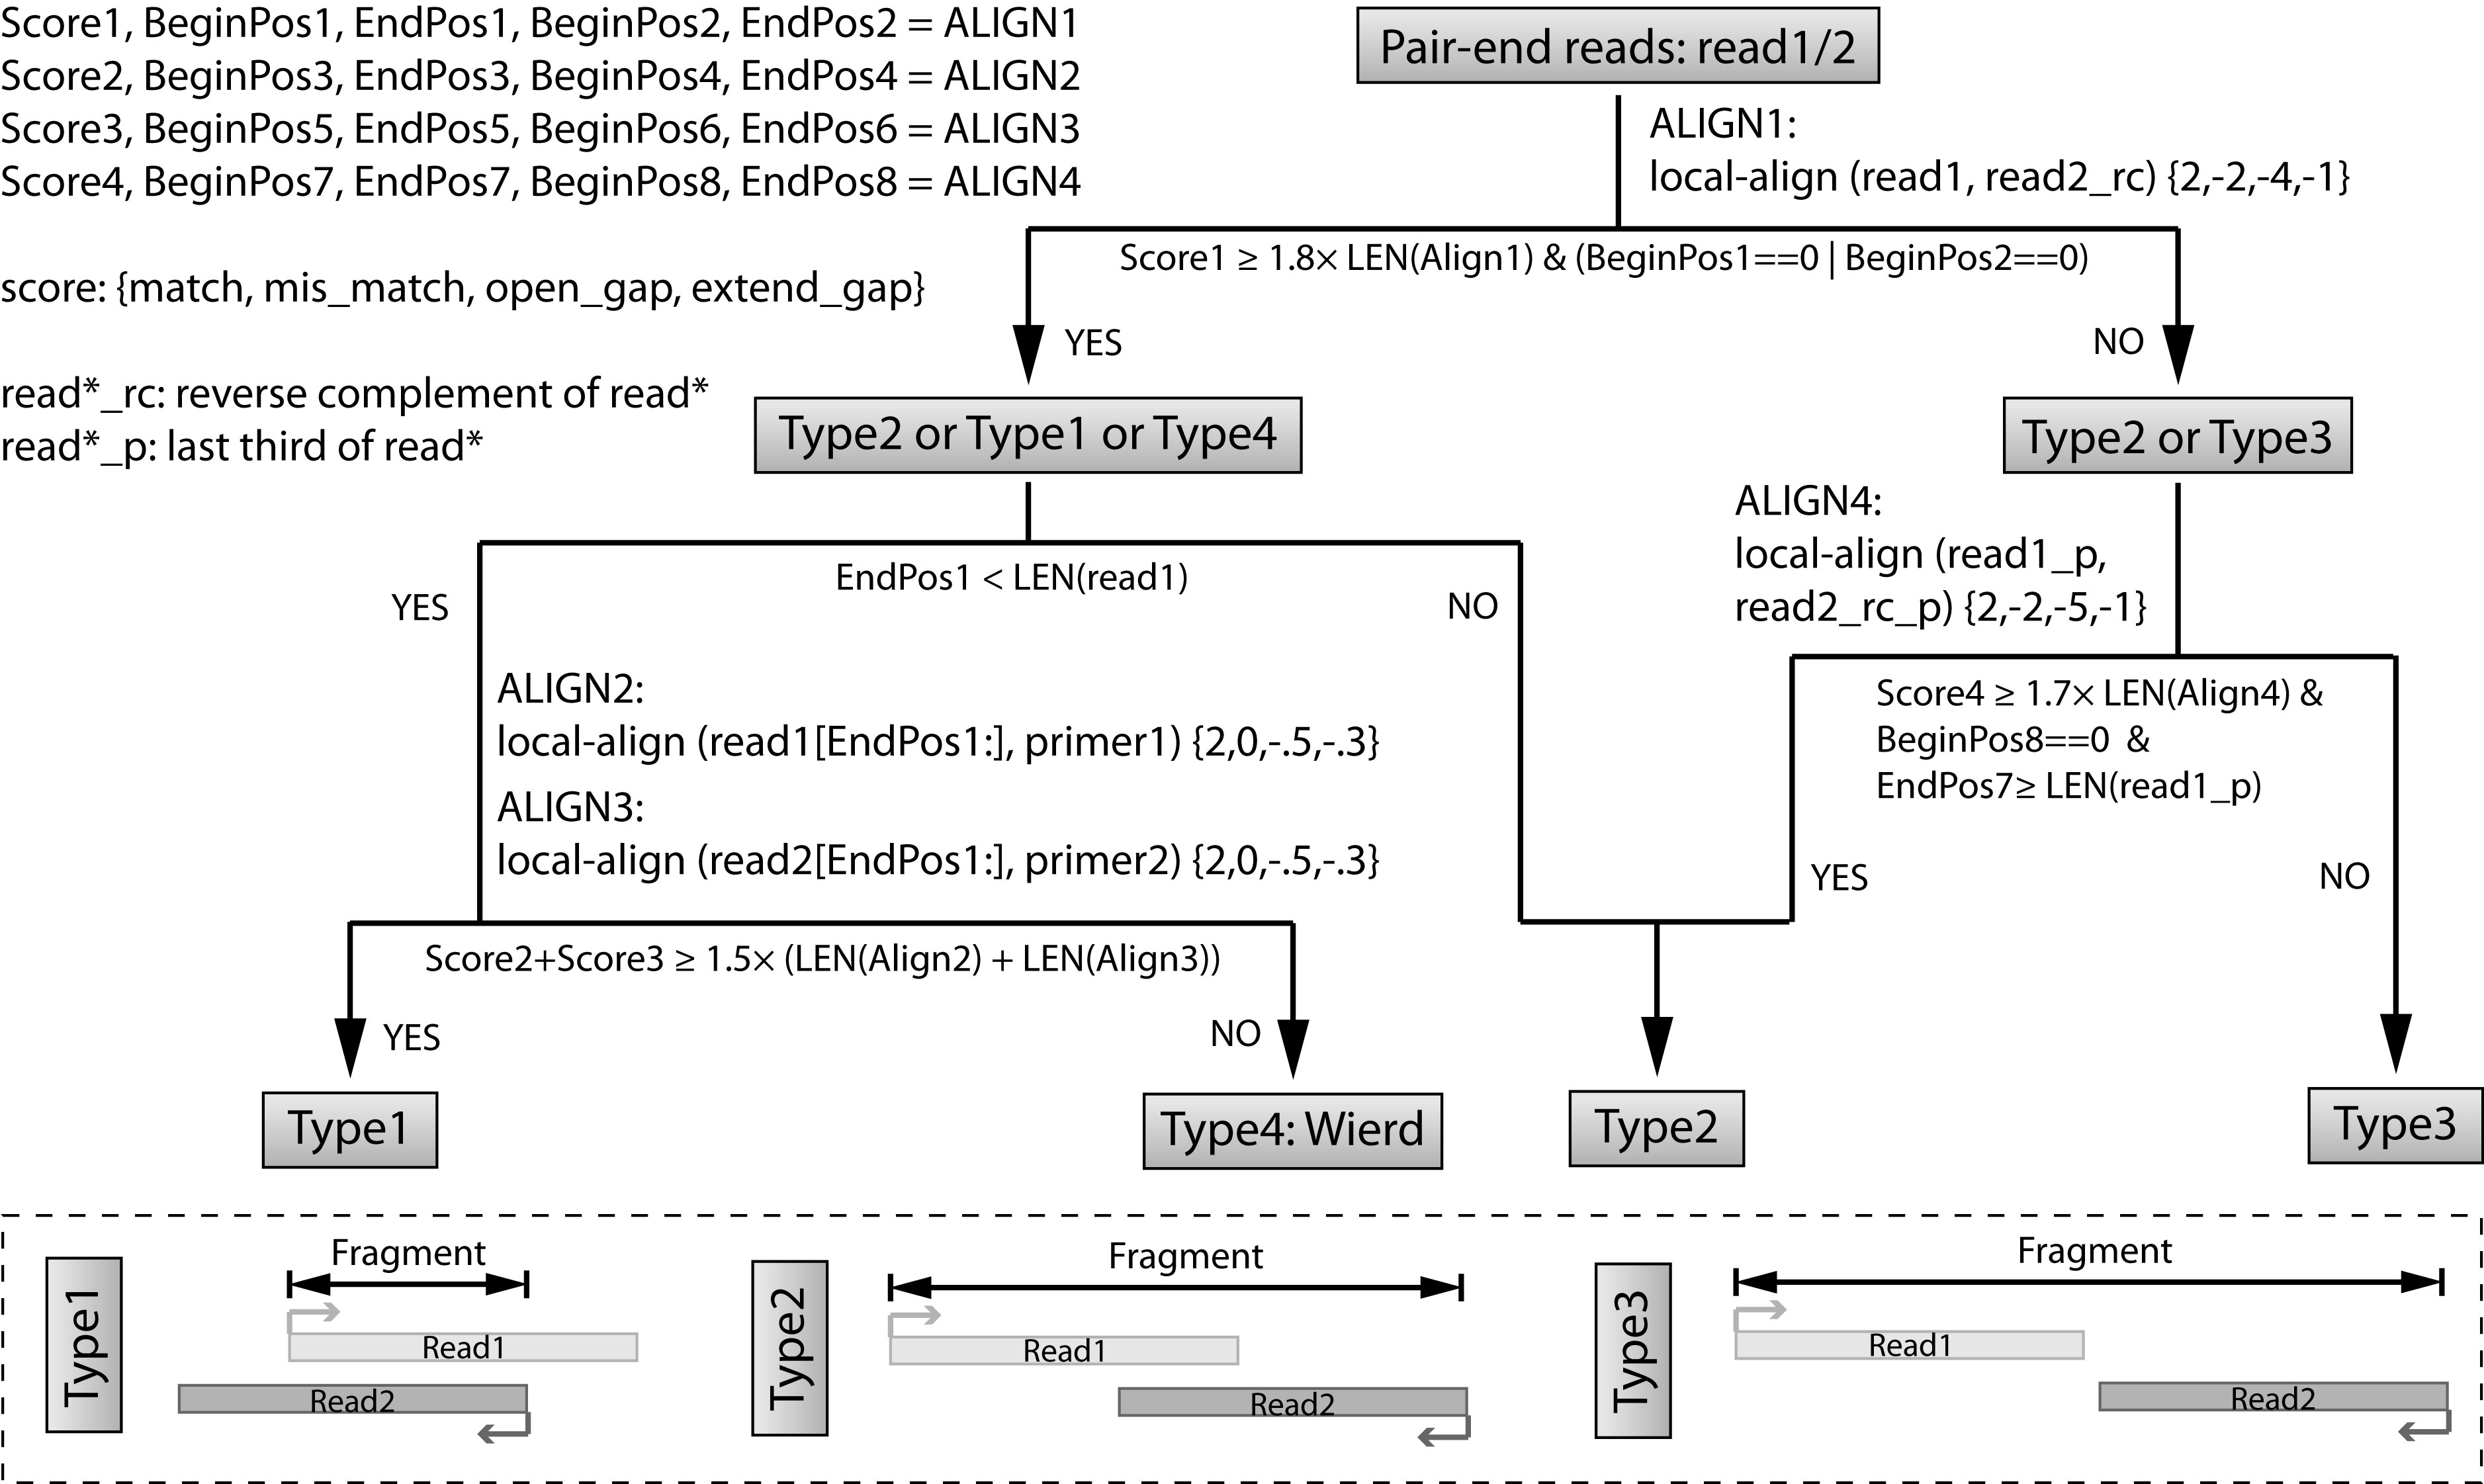
\includegraphics{workflow_for_recoverFragment.jpg}

We will use a complied program \code{recoverFragment} to do that

\begin{Verbatim}[commandchars=\\\{\}]
recoverFragment - recover fragment into 4 different categories from pair-end seq data
=====================================================================================

SYNOPSIS

DESCRIPTION
    -h, --help
          Displays this help message.
    --version
          Display version information
    -I, --inputs STR
          input of forward and reverse fastq file, path of two files separated by SPACE
    -p, --primer STR
          fasta file contianing two primer sequences
    -v, --verbose
          print alignment information for each alignment

EXAMPLES
    recoverFragment -I read\_1.fastq read\_2.fastq -p primer.fasta
          store fragment using fasta/fastq into 4 output files
          'short\_*', 'long\_*','evenlong\_*','wierd\_*'

VERSION
    recoverFragment version: 0.1
    Last update August 2013
\end{Verbatim}


\subsection{Step 4: Split partners and classify different types of fragments.}
\label{Analysis_pipeline:step4}\label{Analysis_pipeline:step-4-split-partners-and-classify-different-types-of-fragments}
When we recovered the fragments, the next we are goting to do is to find parts that are seprarated by the linkers, and from here, we will be able to classify the fragments into different types: ``IndexOnly'', ``NoLinker'', ``LinkerOnly'', ``BackOnly'', ``FrontOnly'', ``Paired''. (see the figure below).

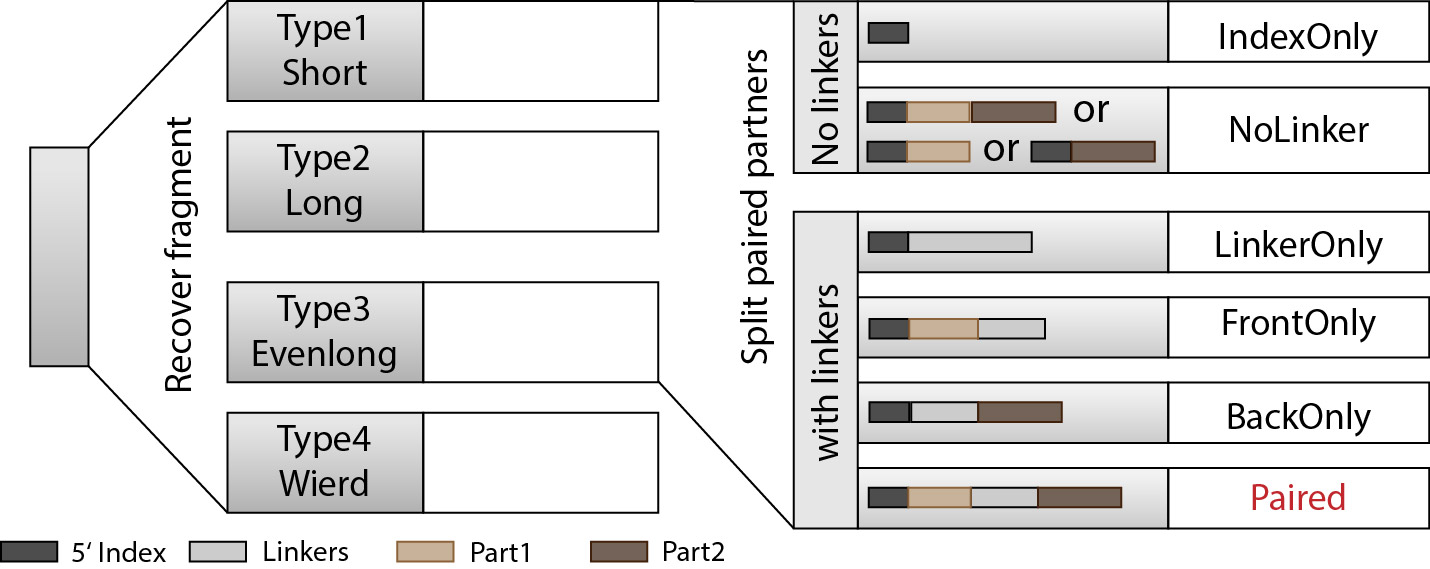
\includegraphics{summary.jpg}

This will be done by \code{split\_partner.py}

\begin{Verbatim}[commandchars=\\\{\}]
usage: split\_partner.py [-h] [-e EVALUE] [--linker\_db LINKER\_DB]
                        [--blast\_path BLAST\_PATH] [-o OUTPUT] [-t TRIM]
                        [-b BATCH] [-l LENGTH]
                        input type3\_1 type3\_2

DESCRIPTION: Run BLAST, find linker sequences and split two parts connected by
linkers

positional arguments:
  input                 the input fasta file containing fragment sequences of
                        type1 and type2
  type3\_1               read\_1 for evenlong (type3) fastq file
  type3\_2               read\_2 for evenlong (type3) fastq file

optional arguments:
  -h, --help            show this help message and exit
  -e EVALUE, --evalue EVALUE
                        cutoff evalues, only choose alignment with evalue less
                        than this cutoffs (default: 1e-5).
  --linker\_db LINKER\_DB
                        BLAST database of linker sequences
  --blast\_path BLAST\_PATH
                        path for the local blast program
  -o OUTPUT, --output OUTPUT
                        output file containing sequences of two sepatated
                        parts
  -t TRIM, --trim TRIM  trim off the first this number of nt as index,
                        default:10
  -b BATCH, --batch BATCH
                        batch this number of fragments for BLAST at a time.
                        default: 100000
  -l LENGTH, --length LENGTH
                        shortest length to be considered for each part of the
                        pair, default: 15

Library dependency: Bio, itertools
\end{Verbatim}

The linker fasta file contain sequences of all linkers

\begin{Verbatim}[commandchars=\\\{\}]
\textgreater{}L1
CTAGTAGCCCATGCAATGCGAGGA
\textgreater{}L2
AGGAGCGTAACGTACCCGATGATC
\end{Verbatim}

The output fasta files will be the input file name with different prefix (``NoLinker'', ``LinkerOnly'', ``BackOnly'', ``FrontOnly'', ``Paired'') for different types. The other output file specified by \code{-o} contains information of aligned linker sequences for each Type1/2 fragment.

For example, if the commend is

\begin{Verbatim}[commandchars=\\\{\}]
split\_partner.py fragment\_ACCT.fasta evenlong\_ACCTRm\_dupPE\_stitch\_seq\_1.fastq
evenlong\_ACCTRm\_dupPE\_stitch\_seq\_2.fastq
-o fragment\_ACCT\_detail.txt --linker\_db linker.fa
\end{Verbatim}
\begin{description}
\item[{Then, the output files will be:}] \leavevmode\begin{itemize}
\item {} 
backOnly\_fragment\_ACCT.fasta

\item {} 
NoLinker\_fragment\_ACCT.fasta

\item {} 
frontOnly\_fragment\_ACCT.fasta

\item {} 
Paired1\_fragment\_ACCT.fasta

\item {} 
Paired2\_fragment\_ACCT.fasta

\item {} 
fragment\_ACCT\_detail.txt

\end{itemize}

\end{description}

The format of the last output file \code{fragment\_ACCT\_detail.txt} will be ``Name \textbar{} linker\_num \textbar{} linker\_loc \textbar{} Type \textbar{} linker\_order''. Here are two examples:

\begin{Verbatim}[commandchars=\\\{\}]
HWI-ST1001:238:H0NYEADXX:1:1101:10221:1918      L1:2;L2:1  19,41;42,67;68,97       None    L2;L1;L1
HWI-ST1001:238:H0NYEADXX:1:1101:4620:2609       L1:2 28,46;47,79     Paired  L1;L1
\end{Verbatim}

In the \textbf{first} fragment, there are three regions can be aligned to linkers, 2 for L1 and 1 for L2, the order is L2, L1, L1. And they are aligned in region {[}19,41{]}, {[}42,67{]}, {[}68,97{]} of the fragment. ``None'' means this fragment is either `LinkerOnly' or `IndexOnly' (in this case it is `LinkerOnly'). This fragment won't be written to any of the output fasta files.

In the \textbf{second} fragment, two regions can be aligned to linkers, and they are both aligned to L1. The two regions are in {[}28,46{]}, {[}47,79{]} of the fragment. the fragment is ``Paired'' because on both two sides flanking the linker aligned regions, the length is larger than 15nt. The left part will be writen in \code{Paired1\_fragment\_ACCT.fasta} and the right part in \code{Paired2\_fragment\_ACCT.fasta}


\subsection{Step 5: Align both parts of ``Paired'' fragment to the genome.}
\label{Analysis_pipeline:step-5-align-both-parts-of-paired-fragment-to-the-genome}\label{Analysis_pipeline:step5}

\subsection{Step 6: Determine strong interactions.}
\label{Analysis_pipeline:step6}\label{Analysis_pipeline:step-6-determine-strong-interactions}

\section{Other functions}
\label{Analysis_pipeline:other-functions}

\subsection{Determine the RNA types of different parts within fragments.}
\label{Analysis_pipeline:rna-types}\label{Analysis_pipeline:determine-the-rna-types-of-different-parts-within-fragments}

\subsection{Find linker sequences within the library.}
\label{Analysis_pipeline:find-linker-sequences-within-the-library}\label{Analysis_pipeline:find-linker}

\chapter{Indices and tables}
\label{index:indices-and-tables}\begin{itemize}
\item {} 
\emph{genindex}

\item {} 
\emph{modindex}

\item {} 
\emph{search}

\end{itemize}



\renewcommand{\indexname}{Index}
\printindex
\end{document}
